%%%%%%%%%%%%%%%%% Test frecuentiastas %%%%%%%%%%%%%%%%%%%

\subsection{Applying the Wilcoxon's signed-rank test to our results}

We will apply the Wilcoxon's signed-rank test for each of the measures obtained, namely: ARI, Unsat and Time. We set as null hypothesis $H_0: $ the distribution of $A - B$ is symmetric about $\mu$. However, given that in the case of ARI it is a problem of maximisation, and in the case of Time and Unsat it is a problem of minimisation, we will consider two different alternative hypotheses. In the case of maximization we propose $H_{max}:$ the distribution of $A - B$ is shifted to the left with respect to $\mu$. On the other hand, in the case of minimization we propose $H_{min}:$ the distribution of $A - B$ is shifted to the right with respect to $\mu$. In this way we assume that SHADE+LS is better than BRKGA+LS and we try to prove it.

In this case we set $\mu = 0$, and work with a confidence level of 95\%, which means that the significance level is 0.05 ($\alpha = 0.05$). Table \ref{tab:freqTest} shows the statistical values obtained using Wilcoxon's signed-rank test for each comparison.

\begin{table}[!htp]
	\centering
	\setlength{\tabcolsep}{7pt}
	\renewcommand{\arraystretch}{1.4}
	\begin{tabular}{ccccc}
		\hline
		Measure & $R^{+}$ & $R^{-}$ & P-value & Alternative hypothesis  \\
		\hline
		ARI & 3088 & 1665 & 0.005254 & $H_{max}$ \\
		Time & 4008 & 1042 & 0.0000001723 & $H_{min}$ \\
		Unsat & 3082.5 & 745.5 & 0.0000003838 & $H_{min}$ \\
		\hline
	\end{tabular}
	\caption{Results obtained by the Wilcoxon's signed-rank test for the comparison SHADE vs BRKGA}
	\label{tab:freqTest}
\end{table}

For all three considered measures, $P-value < \alpha$, therefore in all cases we can reject $H_0$ and infer that there are significant differences between the two methods, giving the advantage to SHADE+LS with basis to the proposed alternative hypothesis. In conclusion, we can safely admit that [the] Wilcoxon's signed-rank test provides empirical evidence in favour of SHADE+LS.


-----------------------------------------------


Constrained clustering is an SSL learning method whose goal is to find a partition of the dataset that meets the proper characteristics of a clustering method result, in addition to satisfying a certain constraint set. It has been succesfully applied in many knowledge fields. It has been used to guide the movement of walking robots, as well as in other advanced robotics applications \cite{davidson2005clustering, semnani2016constrained}. In \cite{seret2014new} constrained clustering is presented as a useful tool in the context of applied marketing. Biology has also made use of constrained clustering, being able to detect simultaneous appearances of genes and proteins in biological data bases \cite{segal2003discovering}. In \cite{levy2008structural} a method of segmenting musical audio into separated sections using constrained clustering is described. Constrained clustering has also been useful to classify Internet traffic, which is considered to be one of the most fundamental functionalities in the network management field \cite{wang2014internet}. Electoral district design problems can also be approached using constrained clustering, as shown in \cite{brieden2017constrained}. Lastly, it is mandatory to name the widely known application to GPS data of constrained clustering, presented in \cite{wagstaff2001constrained}.

\subsection{Short Introduction to Iterated Local Search}

Before defining the iterated local search---from now on ILS---,it is necessary to understand the local search and the motivation that leads to designing methods with greater exploratory capacity.

A local search is a procedure that consists of performing an heuristics-guided iterative improvement. Taking as initial state a well defined solution to the problem, the local search uses a neighbor generation operator to explore new solutions. When a solution better than the current one is found, it replaces the current one. In order to evaluate the solutions, the local search uses a function that assigns a value to each one of them, this is known as a target function. ***This value will be better the closer the solution that evaluates the optimal solution.*** 

Both the neighbor generation operator and the target function used by the local search must be defined for each problem. The target function $f(\cdot)$ determines how good the solution achieved is with respect to the purpose of the problem. The neighbor generation operator takes as base a solution to the problem $s$, and generates a new solution $s^\prime$ by modifying some of its components in a local way.

The Algorithm \ref{alg:LS} presents a basic scheme for a local search procedure. It is worth noting that the condition of line 4 must be adapted if the problem to be solved is one of maximization or minimization. In addition, the general scheme considers that the optimization process ends when the current solution is not improved, however the stop condition can be adapted to each problem.

\begin{algorithm}
	\SetNlSty{textbf}{[}{]}
	\SetNlSkip{0.5em}
	\setstretch{1.2}
	\SetKwFunction{GenerateNeighbor}{GenerateNeighbor}
	\SetKwRepeat{Do}{do}{while}
	\KwIn{Initial solution $s$}
	\BlankLine
	\While{$improvement$}{
		$improvement \leftarrow$ \texttt{false} \\
		
		$s^\prime \leftarrow $ \GenerateNeighbor{$s$}
		
		\If{$f(s^\prime) < f(s)$}{
			
			$s \leftarrow s^\prime$\\
			$improvement \leftarrow$ \texttt{true} \\
			
		}	
	}
	\BlankLine
	\KwRet ($s$)
	
	\caption{Local Search}\label{alg:LS}
\end{algorithm}

With the local search defined in this way, it is easy to see that the solution achieved will be the optimal local $s^*$ closest to the initial solution $s$. Figure \ref{img:LS} shows a pictorical representation of the above.

\begin{figure}[!h]
	\centering
	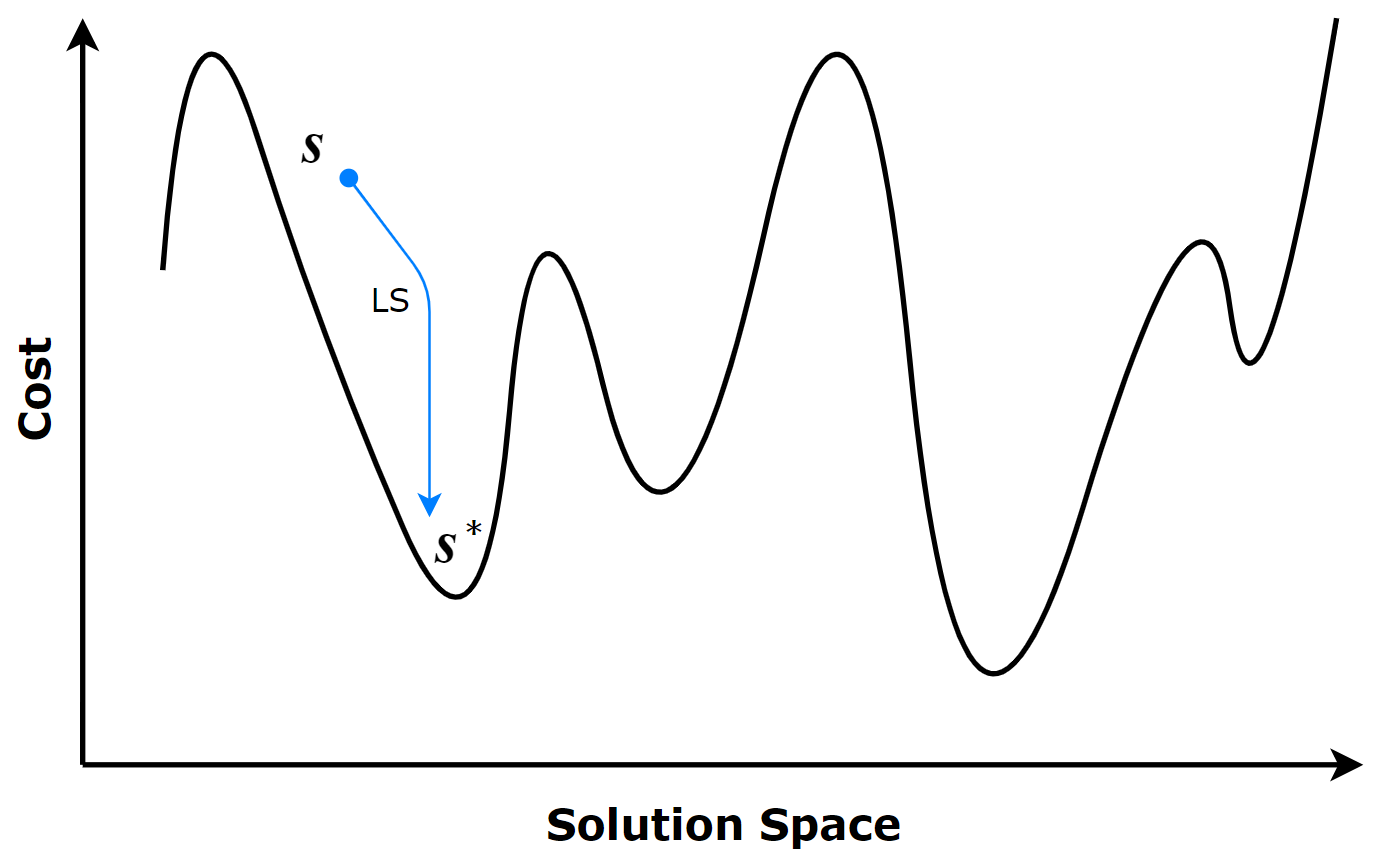
\includegraphics[scale=0.25]{Figures/LS.png}
	\caption{Local optimum achieved by a local search procedure}\label{img:LS}
\end{figure}

It is therefore necessary to appeal to techniques that introduce diversity in the search to avoid the problem of local optimal. This is exactly what ILS is trying to do.

With ILS, once we have reached a local optimum $s^*$, we apply a perturbation to it that, with a high probability, will result in a new solution $s^\prime$ that will not be a local optimum and will be far enough away from $s^*$. After that, we will apply a local search procedure to find a new local optimal $s^{*\prime}$. Figure \ref{img:ILS} shows a representation of the above concepts.

\begin{figure}[!h]
	\centering
	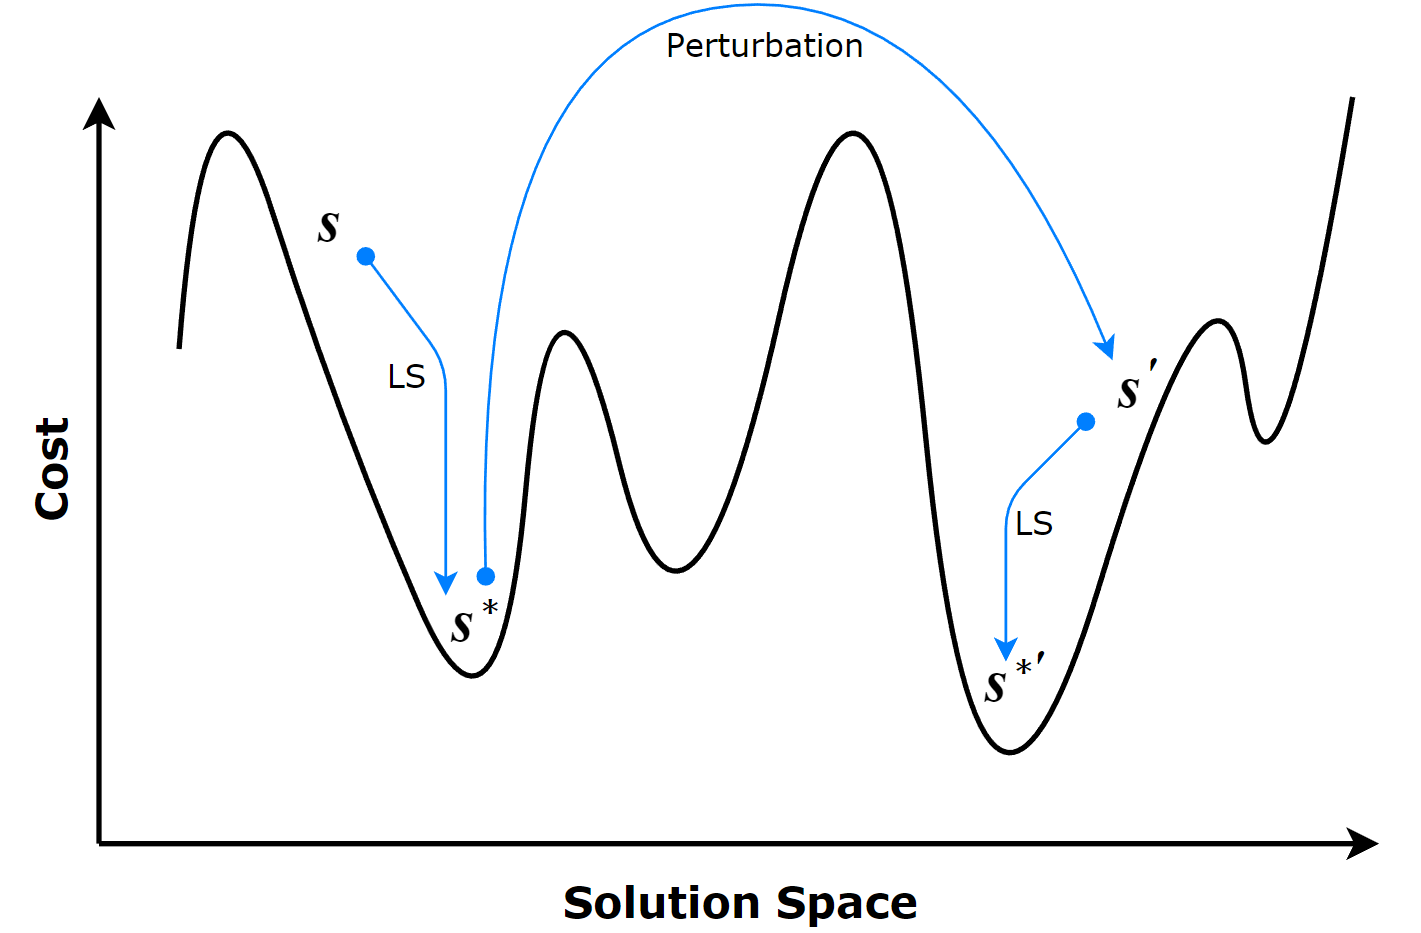
\includegraphics[scale=0.25]{Figures/ILS.png}
	\caption{No se como llamar a esta puta imagen}\label{img:ILS}
\end{figure}

It should be noted that, if the disturbance applied to $s*$ is too small, the most likely is that the local optimum closest to $s^\prime$ is $s^*$ and therefore the solution space will not be explored effectively. On the other hand, if the disturbance is too big, there will be no bias in the generation of new solutions, and therefore the procedure becomes a random reboot-type method.


The method for generating the perturbation applied to the local optimum $s^*$ may vary depending on the problem, and may be based on previous solutions. In this way, it is possible to keep a history of the solutions reached so far, so they can be used when applying the perturbation. Algorithm \ref{alg:ILS} summarizes the ILS overall optimization process.

\begin{algorithm}
	\SetNlSty{textbf}{[}{]}
	\SetNlSkip{0.5em}
	\setstretch{1.2}
	\SetKwFunction{LocalSearch}{LocalSearch}
	\SetKwFunction{Perturbation}{Perturbation}
	\SetKwRepeat{Do}{do}{while}
	\KwIn{Initial solution $s$}
	\BlankLine
	$s^* \leftarrow$ \LocalSearch{$s$}\\
	\While{Termination criteria are not met}{
		
		$s^\prime \leftarrow $ \Perturbation{$s^*$, $history$}\\
		$s^{*\prime} \leftarrow$ \LocalSearch{$s^\prime$}
		
		\If{$f(s^{*\prime}) < f(s^*)$}{
			
			$s^* \leftarrow s^{*\prime}$
			
		}	
	}
	\BlankLine
	\KwRet ($s*$)
	
	\caption{Iterated Local Search}\label{alg:ILS}
\end{algorithm}

In the ILS scheme described in Algorithm \ref{alg:ILS} the acceptance criterion only use the difference in the cost of the solutions to be compared to choose between them. This is the most simple scheme and does not depends on previous solutions recorded in the history.